%% Mapping (chpt5)

The task of mapping was the main challenge of this work. This task consists in determining the 3D coordinates of recognizable features, that can later be used as landmarks by the drone to estimate its own position. The main challenge when building a 3D map using a single monocular camera, is that a point needs to be observed from at least 2 different positions to be mapped. The simplest approach to map a point, is to simply triangulate its position from two different views. We will begin by exploring this approach. We will find that although this does work reasonably well when we are certain of the position of the cameras, it does not when this position is uncertain. In addition, this method does not allow to take more than two views into account. To remedy these problems we will implement a bundle adjustment step, that allows to build a map that is globally consistent. Throughout this section, we will have to make design choices to try to obtain a method that is both fast enough to work in real time, and accurate enough for the drone to control its position. To evaluate these performances, we will perform a standardized test.

\section{Structure of the map}
We will keep the keyframe-based structure for the map from the previous years, but this structure will need to be adapted so that each landmark does not belong to just one keyframe. The map will contain two main data structures: a list of keyframes, and a list of landmarks. Each keyframe will contain the following information: the drone's pose estimation at the moment the keyframe was created, the estimated corrected pose of the keyframe, a list of observed keypoints, meaning their descriptor and their 2D position in the image plane of the keyframe, and for each keypoint, whether it corresponds to a landmark of the map, and which one. Each landmark will contain a descriptor and estimated 3D coordinates.\\
The map grows every time we decide to add a keyframe. When we do, the keypoints of the current image seen by the camera, along with their 2D coordinates and descriptors, are saved in a new keyframe. The descriptors are then matched with descriptors of the other keyframes, and when there is a match between two keypoints of two different keyframes, we can triangulate a new landmark into the map.\\
The main challenges are :\\
- How to triangulate new points?\\
- How to take into account when more than two keyframes see a same keypoint ?\\
- How to prevent errors from accumulating over time?\\


\section{Triangulation}
Our first problem is where to put a landmark in the 3D world from two observations at two different keyframes. If all measurements were perfect, we could simply draw a ray at each keyframe that goes from the camera center and passes through the keypoint in the image plane, and those two rays would intersect at the position of the landmark. \\
Unfortunately, those lines never intersect in practice, due to various errors (measurement errors, errors in the model of the cameras, errors on the position estimation of the cameras), so we need to find a method to locate a 3D point as best as possible from the pair of images.

\begin{figure}[H]
\centering
\vspace{20 mm}
\begin{subfigure}{.5\textwidth}
  \centering
  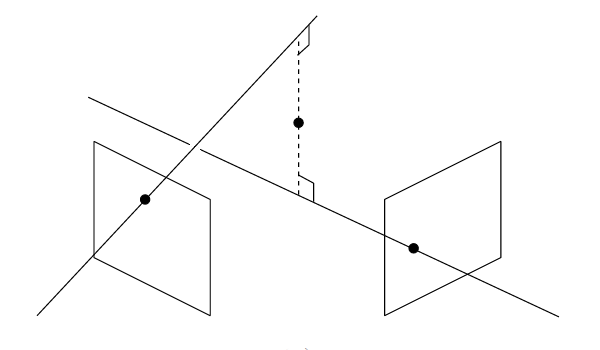
\includegraphics[width=\linewidth]{triang_midpoint.png}
  \caption{Midpoint method}
  \label{fig:midpoint}
\end{subfigure}%
\begin{subfigure}{.5\textwidth}
  \centering
  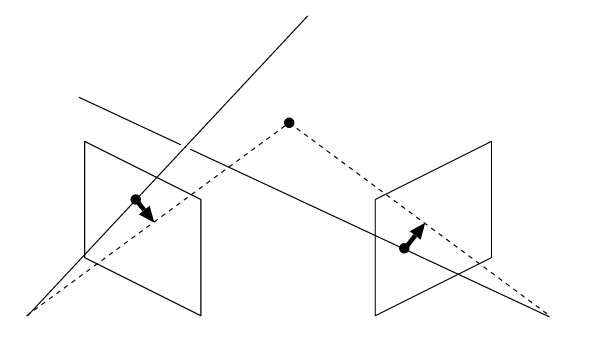
\includegraphics[width=\linewidth]{triang_optimal.png}
  \caption{Optimal Correction}
  \label{fig:optimalcorrection}
\end{subfigure}%

\caption{Triangulation methods}
\label{fig:triang}
\end{figure}

\subsection{Midpoint Method}
The simplest and most obvious solution is to take the midpoint of the common perpendicular of the two rays. This method is intuitive to understand geometrically, and is quite easy to compute. In practice, however its results are not very good, as there is no theoretical reason for this point to be the best.

\subsection{Linear least squares}
A more advanced method for finding the coordinates of a point from a correspondence is called Linear Least squares, and is described in Hartley \& Zisserman's \textit{Multiple view geometry in computer vision} \cite{multipleviewgeometry}.
This method also has the advantage that it is already implemented in the OpenCV library.


\subsection{Optimal Correction}
If we assume that the error on observed points is random and follows a Gaussian distribution with zero mean, then the optimal solution would be to displace the pixels on both images until the resulting rays meet, keeping the displacement of the pixels as small as possible in the least squared sense. Such a solution would give the maximum likelihood estimator of the position of the 3D points, under those assumptions.
There are several algorithms in the literature that triangulate the position of a point using optimal correction. The most popular one, proposed by Hartley and Sturm \cite{hartleysturm}, computes the solution directly but requires finding the root of a 6th degree polynomial. Kanantani et. al.'s method \cite{kanatani} finds a solution iteratively, but requires very few iterations to have an accurate solution, and in practice, is faster than the Hartley Sturm method. It also has better numerical properties, as unlike the Hartley-Sturm method, it does not have singularities at the epipoles.\\
As we will see in the results section (\ref{sec:comparetriang}), optimal correction performs better than the midpoint method, as could be expected. The performance increase from optimal correction is not very big however, because the biggest source of error is not Gaussian noise on the measurements of the points, but errors in the position estimate of the cameras at the moment of creating the keyframes (especially in the robustness test).

\section{Bundle Adjustment}
Having a bad estimation of the keyframe's pose is problematic, as it will result in badly located landmarks, which in turn will cause a bad estimation of the camera's position when future keyframes are created. In the long term, errors will accumulate, and the map will be completely distorted. Luckily, if we have enough point correspondences between two images, it is possible to deduce the relative displacement between the two images. This means that from a set of images, we can reconstruct a scene, without even needing a prior estimation of the position of the cameras that took the images. This is good news as it means that the images can give us some absolute information about the scene, that can be used to correct the errors on the camera poses of the previous keyframes.\\
The problem of adjusting camera poses and 3D point locations in order to minimize the reprojection errors of the 3D points onto the image planes is known as bundle adjustment. As stated above, bundle adjustment has the advantage of being absolute with respect to the world, and so not having errors accumulate. Another advantage of bundle adjustment, is that it can easily take into account points that are seen by more than two cameras, which is not trivial for the triangulation techniques described above. The main disadvantage of bundle adjustment is that it is computationally heavy, so it is important to adapt it to be useable un real time.\\
%TODO move this part:
To show the advantages of bundle adjustment, we compare it with triangulation using the optimal correction method. When using bundle adjustment, optimal correction triangulation is also used to obtain an initial solution, from which we optimize.

Bundle Adjustment an optimization problem of a nonlinear least-squares problem. The problem can be described as follows:

\subsection{Variables and constants}
We are simultaneously trying to determine the layout of the drone's surroundings (landmarks) and to correct the estimations of the drone's poses at the previous keyframe locations. The variables we are optimizing are the previous keyframe poses and the 3D locations of the landmarks. Let $\mathcal{K}$ be the set of keyframes, $\mathcal{L}$ be the set of landmarks and $\mathcal{L}_k$ be the set of landmarks observed by keyframe $k$. We will call the camera centers of the previous keyframes $c_k$ and their roll-pitch-yaw orientation angles $r_k$. The 3D position of the landmarks will be called $p_l$. For each observation of a landmark by a keyframe, we know at what 2D point on he image that point was observed. Let $i_{lk}$ be the image coordinates of landmark $l$ in keyframe $k$.

\begin{table}[H] \caption{Table of notation for Bundle Adjustment}
  \centering
  \begin{tabular}{r c p{10cm} }
  \toprule
  \multicolumn{3}{c}{}\\
  \multicolumn{3}{c}{\underline{Constants}}\\
  \multicolumn{3}{c}{}\\
  $\mathcal{K}$   & $\triangleq$ & Set of keyframes\\
  $\mathcal{L}$   & $\triangleq$ & Set of landmarks\\
  $\mathcal{L}_k$ & $\triangleq$ & Set of landmarks seen by keyframe $k$\\
  $i_{lk}$        & $\triangleq$ & Image coordinates of landmark $l$ in keyframe $k$'s image plane\\
  \multicolumn{3}{c}{}\\
  \multicolumn{3}{c}{\underline{Decision Variables}}\\
  \multicolumn{3}{c}{}\\
  $c_k$           & $\triangleq$ & Position of camera center of keyframe $k$\\
  $r_k$           & $\triangleq$ & Roll-pitch-yaw angles of camera of keyframe $k$\\
  $p_l$           & $\triangleq$ & Position of landmark $l$\\
  \bottomrule
  \end{tabular}
  \label{tab:banotation}
\end{table}

$\mathrm{Proj}_k(\cdot)$ is the projection operator of keyframe $k$, it transforms the 3D point coordinates of any point into the 2D image coordinates of that point if it were perfectly observed by keyframe $k$. This operator depends on the intrinsic (focal length, projection center, skew), and extrinsic (position and orientation) parameters of the camera. In general, bundle adjustment refers to the problem of adjusting both the intrinsic and extrinsic camera parameters of the different keyframes, but in our case, the same camera is used at every location, and the intrinsic parameters have been found in advance using camera calibration. Therefore, we can simplify our model by taking the instrinsic parameters as known constants, and only solving for the extrinsic parameters and the position of the landmarks.

\subsection{Objective function}
We want to minimize the reprojection error of the observed landmarks. After estimating $p_l$, the position of landmark $l$, we can reproject point $l$ into the images it was observed from. For example, $\mathrm{Proj}_k(p_l)$ is the reprojection of point $l$ into the image plane of camera $k$. The projection operator $\mathrm{Proj}_k(\cdot)$ is uniquely defined by the camera's position and orientation (as the intrinsic parameters were fixed in advance). We can then compare the reprojection with the actual observation of point $l$ by camera $k$ to find out how consistent the estimation of the position of point $l$ is with the estimation of the position and orientation of keyframe $k$. Using a least squares loss function, the objective becomes:
\begin{equation}
  \min \sum_{k\in\mathcal{K}}\sum_{l\in\mathcal{L}_k} L(\mathrm{Proj}_k(p_l) - i_{lk})
\end{equation}
for some loss function $L(\cdot)$. We would like to use a squared loss function, as it has good computational properties, but the drawback it gives a lot of weight to outliers. If some landmarks result from bad point correspondences, their reprojection errors will be very large, so they will influence the end result quite a lot. To reduce the effect of outliers, we use a more robust loss function: the Huber loss function.
\begin{equation} \label{eq:huber}
  L_\delta(x) = \left\{ \begin{array}{l l}
    \frac{1}{2} x^2 & \mathrm{if } |x| \leq \delta \\
    \delta|x| - \frac{1}{2}\delta^2 & \mathrm{otherwise} \end{array} \right.
\end{equation}
This function is a parabola for values if $x$ smaller than $\delta$, and a straight line elsewhere.\\

Note that if we kept the keyframe positions and orientations constant, and if there were only 2 keyframes observing each landmark, then the triangulation obtained with optimal correction would already give us the landmark positions that minimize this reprojection error. The interest of using bundle adjustment is that it allows to correct the positions of the camera at the keyframes, and to consider more than two observations per landmark.

\subsection{Constraints}

\subsection{Solver}


\section{Mapping Strategy}

\subsection{Map Initialization} %TODO make this subsection better
Because of the chicken-and-egg nature of SLAM (an estimate of the position is necessary to place landmarks, but a map is necessary to estimate the position), a special procedure is needed to initialize the map. Arbitrarily, we decide to fix the origin of the reference frame to be the at the pose of the drone where it creates first keyframe. However, this first keyframe is not enough to initialize a map, because two views of keypoints are required to triangulate them. THis means we have to fly blindly to the location of the second keyframe before we can initialize the map, and begin to estimate the drone's position using the map and PnP.\\
The only available sensors during this first, blind flight are the IMU, the ultrasonic sensor, and the bottom camera (for optical flow). Of these, only the ultrasonic sensor gives an absolute measurement of position, the others all measure speed, and this speed estimation has to be integrated to give a displacement estimate. For this reason, we will mostly rely on the ultrasonic sensor to estimate the relative position from where we take the second view. Because the ultrasonic sensor only gives the distance from the bottom of the drone to the ground, the drone should fly straight up from its first position (the origin) to reach its second position.\\
Once in its second position, the drone can match seen keypoints from both views, and from its estimated position, triangulate those points to the map. Then, using bundle adjustment, the error in the estimation of the displacement between the two first keyframes can be corrected, to give a better map.

\subsection{Rejecting outliers}
When looking closer at the results of bundle adjustment, we find that a large part of the errors comes from a small number of points. Figure \ref{fig:errorrepartition} shows the repartition of contribution to the objective function between the landmarks as a logarithmic scale. We can see that \SI{1}{\percent} of the landmarks account for more than \SI{40}{\percent} of the total error, and that \SI{10}{\percent} of the landmarks account for more than \SI{80}{\percent} of the total error.  One possible explanation is that these points do not correspond to real world points, so that even if we have the correct position of all cameras exactly, the rays corresponding to these points will not intersect, or even be close to intersection. For this reason, after every bundle adjustment pass, we could look at the contribution of every mapped point to the objective function, and eliminate points whose error is too high. Before doing this, there are some things that we have to take into account, because as a point is observed by an increasingly large number of cameras:
\begin{itemize}
  \item Its total contribution to the cost function will increase, as each observation of a point adds a term to the objective function
  \item Its contribution per observation to the cost function will also increase, because every time an observation is added, the location of the point will change a bit, and its position will become less optimal if we only consider the cameras that already saw the point before.
\end{itemize}
For these reasons, we will put a different threshold on the points depending on the number of keyframes that see the point. If a point is seen by a large number of keyframes, we will allow it to have larger errors in the objective function before removing it.


\begin{figure}[H]
  \centering
  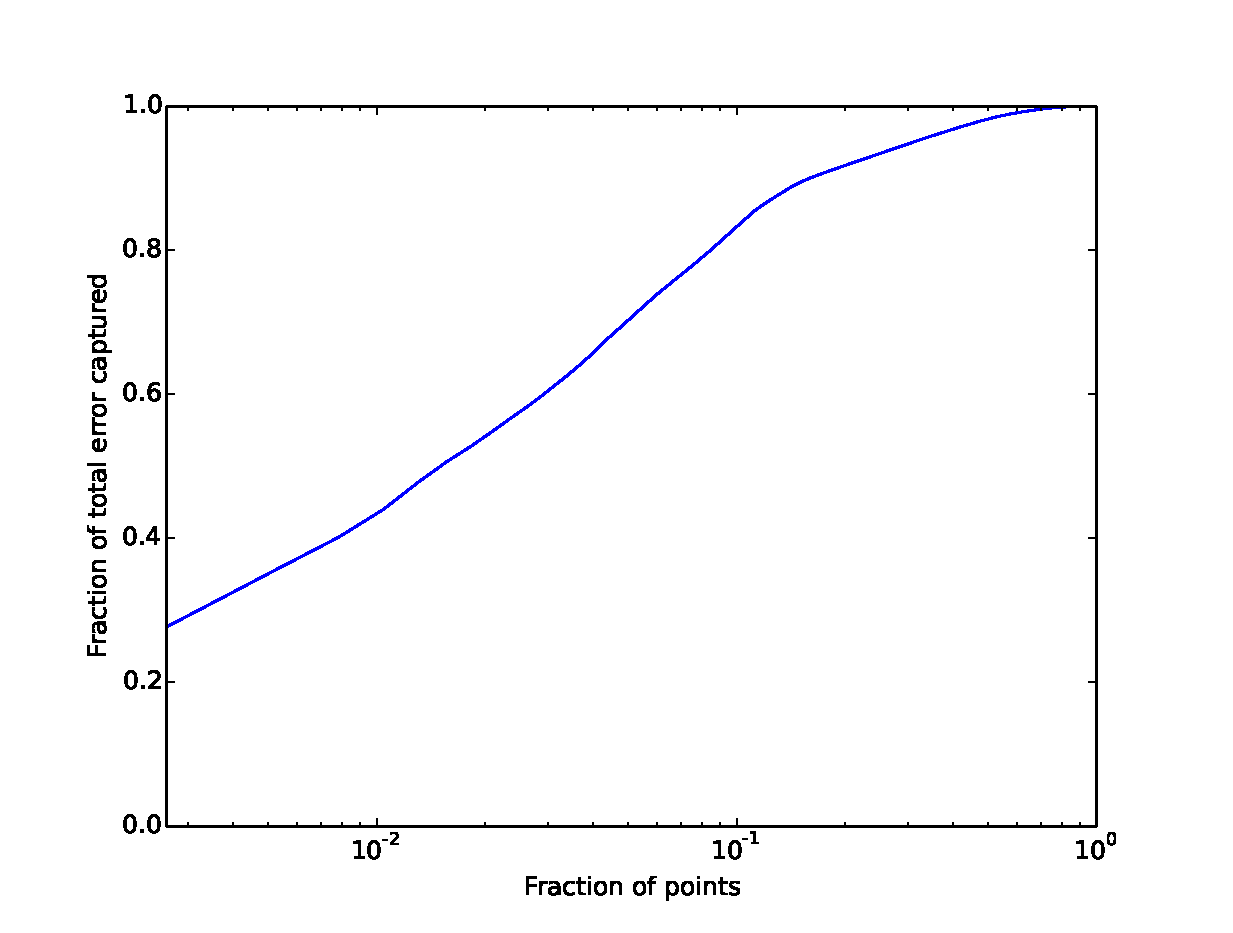
\includegraphics[scale=0.6]{err_repartition_4.eps}
  \caption{Repartition of error among points}
  \label{fig:errorrepartition}
\end{figure}
